\begin{figure}[htbp]
    \centering
    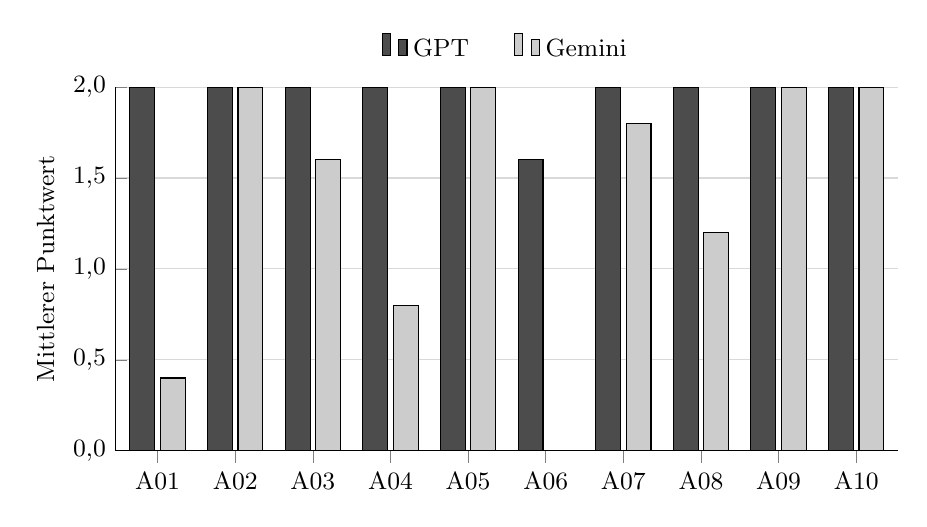
\begin{tikzpicture}
    \begin{axis}[
        width=0.95\textwidth,
        height=6.2cm,
        ybar=2pt,
        bar width=9pt,
        ymin=0, ymax=2,
        ytick={0,0.5,1,1.5,2},
        yticklabels={0{,}0, 0{,}5, 1{,}0, 1{,}5, 2{,}0},
        ylabel={Mittlerer Punktwert},
        ylabel style={font=\small},
        symbolic x coords={A01,A02,A03,A04,A05,A06,A07,A08,A09,A10},
        xtick=data,
        tick label style={font=\small},
        enlarge x limits=0.06,
        ymajorgrids=true,
        grid style={draw=black!15},
        axis lines*=left,
        legend style={
            at={(0.5,1.04)}, anchor=south,
            legend columns=2, draw=none, font=\small,
            /tikz/every even column/.append style={column sep=0.5cm}
        },
    ]

    \addplot[draw=black, fill=black!70] coordinates {
        (A01,2.00) (A02,2.00) (A03,2.00) (A04,2.00) (A05,2.00)
        (A06,1.60) (A07,2.00) (A08,2.00) (A09,2.00) (A10,2.00)
    };
    \addlegendentry{GPT}

    \addplot[draw=black, fill=black!20] coordinates {
        (A01,0.40) (A02,2.00) (A03,1.60) (A04,0.80) (A05,2.00)
        (A06,0.00) (A07,1.80) (A08,1.20) (A09,2.00) (A10,2.00)
    };
    \addlegendentry{Gemini}

    \end{axis}
    \end{tikzpicture}
    \caption[Ergebnisse der faktischen Fragen]%
    {Mittlere Punktwerte von GPT und Gemini für die zehn faktischen Fragen der Kategorie~A über jeweils fünf Wiederholungen. Der maximal erreichbare Punktwert beträgt 2.}
    \label{fig:kategorie-a-ergebnisse}
\end{figure}